
\section{Pristupanje igri}

Nakon pokretanja programa na zaslonu korisnika prikazuje se grafičko korisničko sučelje (prikazano na slici 1.) na kojemu je prikazano: tipka za prikaz top liste najboljih igrača, tipka za igranje nove igre gdje se prikazuje forma za registraciju i logiranje u aplikaciju, tipka za prikaz pravila igre. Pritiskom na tipku za prikaz top liste najboljih igrača korisniku se prikazuje tablica (slika 2.) na kojoj se mogu vidjeti broj pobjeda, broj poraza, ukupan broj igara i omjer pobjeda i poraza svakog igrača.\newline

Tablica je sortirana po omjeru pobjeda i poraza svakog igrača pa je tako na vrhu prikazan igrač sa najboljim omjerom. Kada korisnik pritisne tipku za pokretanje nove igre, otvara se mogućnost da se registrira kao novi korisnik ukoliko ne posjeduje račun s odgovarajućim korisničkim imenom i lozinkom. Ista se forma prikazuje (slika 3.) i za prijavu i za registraciju novog korisnika aplikacije jer program sam prepoznaje postoji li u bazi korisnik sa upisanim korisničkim imenom i lozinkom.\newline 

Ako ne postoji račun sa nekim korisničkim imenom, onda program uspješno registrira novog korisnika. U suprotnom ako već postoji račun sa nekim korisničkim imenom, onda program dozvoljava registraciju samo za jednom lozinkom, inače šalje upozorenje da je lozinka pogrešna. Pritiskom na tipku pravila korisnik dobiva kratki prikaz najvažnijih pravila ove igre, što je i prikazano na donjim slikama.


\begin{figure}[H]
\centering
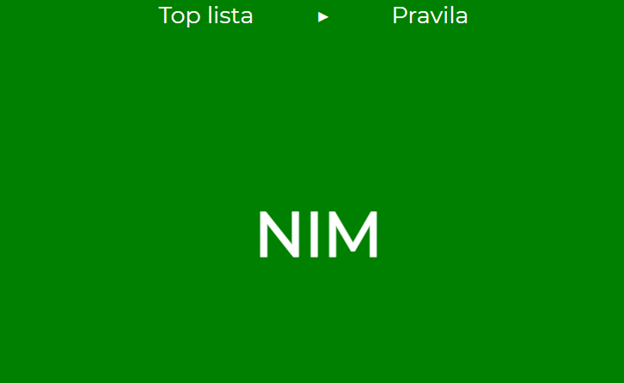
\includegraphics[width=14cm]{slike-program/Slika1.png}
\caption{Stanje programa nakon pokretanja.}
\label{}
\end{figure}

\begin{figure}[H]
\centering
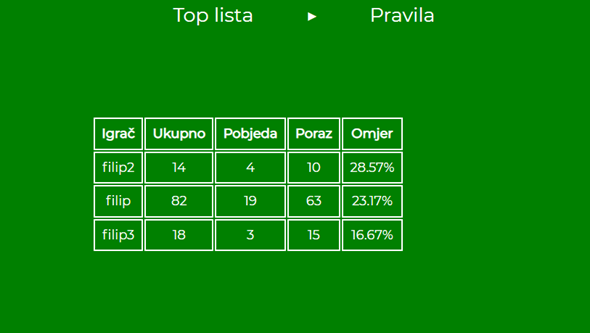
\includegraphics[width=14cm]{slike-program/Slika2.png}
\caption{Stanje programa nakon pritiska na tipku top lista.}
\label{}
\end{figure}

\begin{figure}[H]
\centering
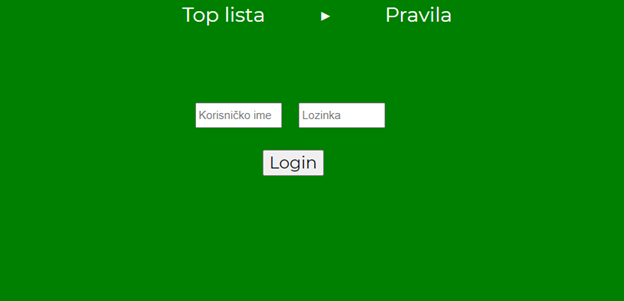
\includegraphics[width=14cm]{slike-program/Slika3.png}
\caption{Forma za prijavu/registraciju korisnika.}
\label{}
\end{figure}

\begin{figure}[H]
\centering
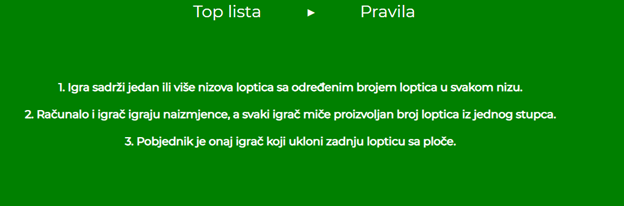
\includegraphics[width=14cm]{slike-program/Slika4.png}
\caption{Prikaz pravila igre.}
\label{}
\end{figure}


Nakon uspješnog ulaska u svoj profil korisniku se prikazuje forma na kojoj odlučuje hoće li on ili računalo biti prvi na potezu i koliko će stupaca loptica sadržavati igra. Na početku je zadano da je korisnik prvi na potezu i da se ploča sastoji od 5 stupaca loptica (stupci sadrže po 1,2,3,4 i 5 loptica). Broj stupaca može biti između 2 i 10, u suprotnom korisnik dobiva upozorenje da je neispravna veličina ploče. Kada je korisnik zadovoljan sa postavljenim početnim postavkama i kada su postavke ispravne korisnik može započeti novu igru pritiskom na donju tipku, a ako želi odustati u gornjem desnom dijelu može pritisnuti na tipku za izlaz.

\begin{figure}[H]
\centering

\includegraphics[width=14cm]{slike-program/Slika5.png}
\caption{Prikaz forme za pokretanje nove igre.}
\label{}
\end{figure}


\section{Prikaz igre}

Nakon pokretanja nove igre na zaslonu korisnika prikazuje se grafičko korisničko sučelje (prikazano na slici 6.) na kojemu je prikazano koji je igrač trenutno na potezu i ispod toga trenutno stanje ploče za igru, odnosno broja loptica koji još nisu uklonjeni iz igre. Na slici je prikazana nova igra po početno zadanim postavkama na prvoj stranici igre.  Prelaženjem miša preko loptica one postaju bijele i time korisnik vidi koje će loptice tim potezom ukloniti. Uklanjanjem miša od loptica one ponovno postaju sive, a klikom na loptice korisnik čini svoj potez u igri čime se oni više ne vide na ploči i time prepušta računalu da izvrši svoj sljedeći potez. Korisnik u jednom potezu može ukloniti loptice samo iz jednog stupca. Korisnik i računalo se međusobno izmjenjuju sve dok se zadnja loptica ne ukloni sa ploče.\newline

 Cilj ove igre je natjerati protivničkog igrača da on ne uklanja zadnju lopticu sa ploče pa je u tom slučaju on gubitnik u igri. Nakon što ploča ostane bez ijedne loptice sukladno gore navedenim pravilima prikazuje se poruka da je korisnik pobijedio ili u drugom slučaju izgubio igru (prikazano na slici 7. i 8.) i ispod toga gumb za pokretanje nove igre. Gumb za povratak na početnu stranicu je također prikazan u gornjem desnom dijelu u slučaju da korisnik nakon igre želi odustati i izaći iz programa. U slučaju da korisnik pritisne tipku za izlaz iz programa dok je igra pokrenuta prikazuje se upozorenje da igra još traje, što znači da korisnik ako želi odustati od igre prvo mora pritisnuti donju tipku za izlaz kako bi završio igru, a tek onda izaći iz programa kako bi se pokrenuta igra uspješno završila.


\begin{figure}[H]
\centering
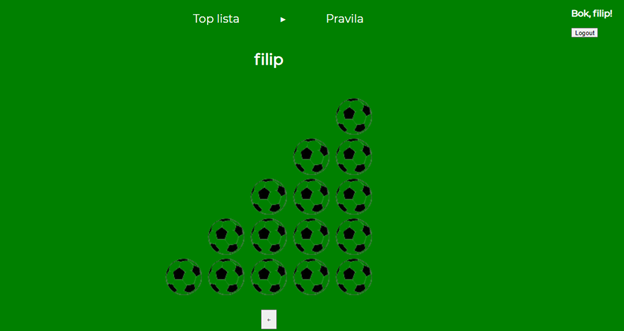
\includegraphics[width=14cm]{slike-program/Slika6.png}
\caption{Stanje programa nakon odabira tipke za početak nove igre.}
\label{}
\end{figure}

\begin{figure}[H]
\centering

\includegraphics[width=14cm]{slike-program/Slika7.png}
\caption{Stanje programa nakon pobjede igrača.}
\label{}
\end{figure}

\begin{figure}[H]
\centering

\includegraphics[width=14cm]{slike-program/Slika8.png}
\caption{Stanje programa nakon poraza igrača.}
\label{}
\end{figure}